\documentclass{book}

\usepackage[spanish]{babel}
\usepackage[utf8]{inputenc}

\usepackage{graphicx}
\usepackage{lipsum}
\usepackage{microtype}

\usepackage[T1]{fontenc}
\usepackage{lmodern}

\usepackage[pdftex]{hyperref}

\hypersetup{pdfauthor={J. S. Castellanos-Durán},pdftitle={RECANEWS Volumen 3 - Marzo 2015},colorlinks,linkcolor=black,urlcolor=blue}

\usepackage[paperwidth=210mm, paperheight=297mm, textwidth=160mm, textheight=240mm, bindingoffset=1cm]{geometry}


% obliczenie szerokości lewego marginesu
\usepackage{calc}
\newlength{\lmargin}
\setlength{\lmargin}{1in + \hoffset + \oddsidemargin}

\usepackage{flowfram}

\usepackage{color}

\usepackage{tikz}
\usepackage{anyfontsize}

% definicja ramek typu flow umieszczonych na stonie 1
\newflowframe[1]{8cm}{24\baselineskip}{-.50cm}{0\baselineskip}[frame1-1a]
\newflowframe[1]{8cm}{23\baselineskip}{8.5cm}{0\baselineskip}[frame1-2b]
%\newflowframe[1]{5cm}{27\baselineskip}{11cm}{0\baselineskip}[frame1-3c]

%definicja ramek statycznych wstawianych na stronie 1
\newstaticframe[1]{\paperwidth}{14cm}{-\lmargin}{12.5cm}[frameS-1a]
\newstaticframe[1]{14cm}{7\baselineskip}{0cm}{45\baselineskip}[frameS-1b]

%definicja ramki dymamicznej wstawiania na stonie nieparzystej
\newdynamicframe[odd]{2cm}{2cm}{-\lmargin}{6cm}[frameD-1a]
%definicja ramki dymamicznej wstawiania na stonie parzystej
\newdynamicframe[even]{2cm}{2cm}{\textwidth+\lmargin-2cm}{6cm}[frameD-1b]

% definicja ramek typu flow na kolejnych stronach
\newflowframe[>1]{8cm}{57\baselineskip}{-.50cm}{0\baselineskip}[frame2-1a]
\newflowframe[>1]{8cm}{57\baselineskip}{8.5cm}{0\baselineskip}[frame2-2a]
%\newflowframe[>1]{5cm}{57\baselineskip}{11cm}{0\baselineskip}[frame2-3a]

\definecolor{green}{rgb}{0.6,0.8,0.1}

\title{RECANEWS Volumen 3 - Marzo 2015}
\author{J. Sebastián Castellanos Durán}
\date{\relax}

\begin{document}

\pagestyle{empty}

% wstawienie numerów stron w ramki dynamiczne frameD-1a i frameD-1b
\begin{dynamiccontents*}{frameD-1a}
\begin{tikzpicture}
\draw(0,0) node [fill=orange, minimum width=2cm, minimum height=2cm]{
{\sffamily\bfseries\Huge\color{white}\thepage}
};
\end{tikzpicture}
\end{dynamiccontents*}

\begin{dynamiccontents*}{frameD-1b}
\begin{tikzpicture}
\draw(0,0) node [fill=orange, minimum width=2cm, minimum height=2cm]{
{\sffamily \bfseries\Huge\color{white}\thepage}
};
\end{tikzpicture}
\end{dynamiccontents*}


% wstawienie grafiki w ramkię statyczną frameS-1a
\begin{staticcontents*}{frameS-1a}
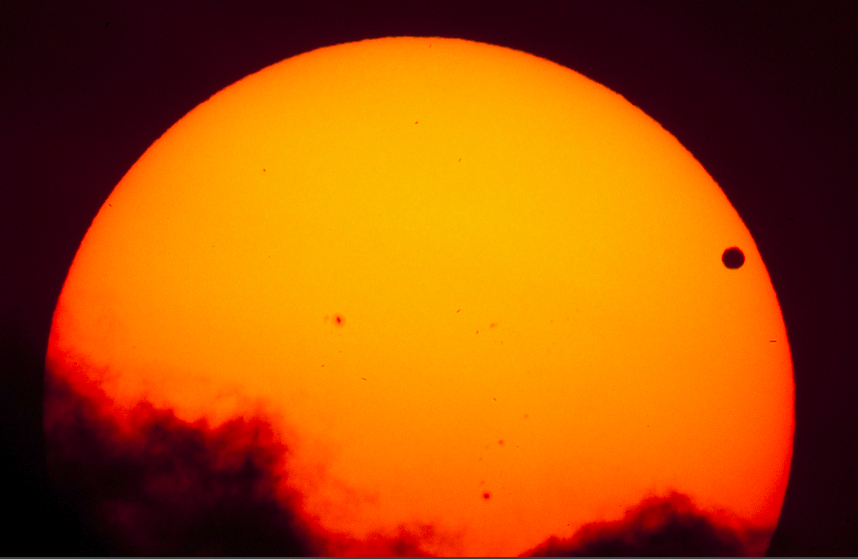
\includegraphics[width=1\textwidth]{fig11.jpg}
\end{staticcontents*}

% wypełnienie tekstem ramki statycznej frameS-1b
\begin{staticcontents*}{frameS-1b}
\begin{tikzpicture}
\draw(0,0) node [fill=white, text width=13cm, inner sep=5mm, opacity=0.7]{
\large\sffamily
{\fontsize{70}{30}\selectfont {\color{black} RECANEWS}}\\


{\fontsize{30}{30}\selectfont {\color{black} Volumen 3}}\\
\begin{center}
{\fontsize{30}{30}\selectfont {\color{black} Llamada a publicaciones}}\\
\end{center}
\begin{flushright}
{\fontsize{30}{30}\selectfont {\color{black} Marzo 2015}}
\end{flushright}
};
\end{tikzpicture}
\end{staticcontents*}


%\tableofcontents{}
% wlanie tekstu do wszystkich ramek typu flow



\newpage


\renewcommand\thesection{\arabic{section}}
\renewcommand\thesubsection{\arabic{subsection}}

%*********************************************
\addcontentsline{toc}{section}{Propósito}
\section*{Propósito}
%*********************************************
Esta iniciativa fue propuesta en el COCOA IV realizado en Pasto a inicios de Diciembre, 2014. La idea de este medio de comunicación entre los estudiantes y personas que trabajan en astronomía en Colombia o en el exterior es contar con alternativas para el fortalecimiento de la Comunidad, para entablar interacción entre las personas que trabajan en ciencias del  espacio, facilitar posibles colaboraciones y conocer qué se está realizando en los diferentes grupos de investigación y demás instancias donde se cuente con presencia de científicos colombianos a nivel nacional y en el exterior. \\
\\
También, este canal puede ser usado para la divulgación de eventos, escuelas, deadlines para aplicaciones a programas, pasantías y demás instancias que pueden interesar a los integrantes de la comunidad.  \\
\\
Por último, este espacio puede ser usado para avisos de trabajo y estado del arte de la astronomía en Colombia, noticias sobre proyectos, publicaciones de artículos, estado de la Agencia Colombiana del Espacio y cualquier tipo de publicación que pudiese interesar a astrónomos y personas en áreas relacionadas en Colombia.

%*********************************************
\addcontentsline{toc}{section}{¿Quién puede publicar?}
\section*{¿Quién puede publicar?}
%*********************************************
Este es medio de comunicación es totalmente libre para su publicación. De esta manera, cualquier persona interesada en publicar debe enviar su publicación antes del 25 de cada mes.

%*********************************************
\addcontentsline{toc}{section}{¿Qué se puede publicar?}
\section*{¿Qué se puede publicar?}
%*********************************************
\begin{itemize}
\item Noticias de Astronomía y ciencias del espacio en Colombia.
\item Eventos de Astronomía y ciencias del espacio.
Colaboraciones (e.g. necesidad de tiempo en clusters).
\item Charlas de Astronomía y ciencias del espacio.
\item Publicaciones de Astronomía y ciencias del espacio de colombianos.
\item Artículos del estado del arte de la Astronomía y ciencias del espacio en Colombia (e.g. Noticias sobre investigaciones, avances de los proyectos de telescopios colombianos, de LAGO, etc).
\item Deadlines para aplicaciones a programas, pasantías, escuelas, congresos, en Astronomía y ciencias del espacio  en colombia y en el exterior.
\item Oportunidades de trabajo en Astronomía y ciencias del espacio  en colombia y en el exterior.
\item Cualquier información importante en temas de Astronomía y ciencias del espacio  en colombia y en el exterior.
\end{itemize}


%*********************************************
\addcontentsline{toc}{section}{¿Cuál es la periodicidad de RECANEWS?}
\section*{¿Cuál es la periodicidad de RECANEWS?}
%*********************************************

Esta publicación se realizará mensualmente a principios de cada mes (siempre y cuando haya alguna publicación). También se hará una llamada para publicaciones a mediados de cada mes. 

%*********************************************
\addcontentsline{toc}{section}{¿Cómo publicar en RECANEWS?}
\section*{¿Cómo publicar en RECANEWS?}
%*********************************************

Para publicar en RECANEWS se debe enviar un correo a reca.news@gmail.com con las siguientes especificaciones:
\begin{description}
\item[Correo:]\url{reca.news@gmail.com}
\item[Asunto:]Título de la publicación
\item[Contenido:]Contenido de la publicación\\
Persona encargada (Opcional)\\
Correo de la persona encargada (Opcional)
\end{description}
  

%*********************************************
\addcontentsline{toc}{section}{¿Quién recibe RECANEWS?}
\section*{¿Cómo publicar en RECANEWS?}
%*********************************************

Cualquier persona interesada en hacer parte de la base de datos puede enviar un correo a 
\begin{description}
\item[Correo:]\url{reca.news@gmail.com}
\item[Asunto:]Subcripción a RECANEWS
\item[Contenido:]Correo (Obligatorio).\\
Nombre o nickname (opcional)
\end{description}

%*********************************************
\addcontentsline{toc}{section}{Repositorio de RECANEWS}
\section*{Repositorio de RECANEWS}
%*********************************************

Repositorio: \url{https://github.com/recanews}\\



%*********************************************
\addcontentsline{toc}{section}{Contacto del RECA}
\section*{Contacto del RECA:}
%*********************************************

\begin{description}
\item[Correo RECA:]\url{reca.astronomia@gmail.com}
\item[Facebook:] \url{https://www.facebook.com/RECAstronomia}
\item[Google$+$:] \url{http://goo.gl/P0DEf4}
\item[Twitter:] \url{https://twitter.com/RECAstronomia}
\item[Pagina Web:] \url{http://goo.gl/Fl4zQP}
\end{description}


%*********************************************
\addcontentsline{toc}{section}{Representantes de RECA en las regiones}
\section*{Representantes de RECA en las regiones}
%*********************************************
\begin{description}
\item[Medellín:]Malory Agudelo Vásquez\\
\url{magudelov@gmail.com}\\ \url{magudelov@fisica.udea.edu.co}
\item[Pereira:]Luisa Fernanda Cardona\\ \url{luisferncardona@utp.edu.co}
\item[Pasto:]Katherine Mafla Oliva\\
\url{skmofis13@gmail.com}
\item[Cali:]Daniel Santacruz\\
\url{santacruz121@gmail.com}
\item[Bogotá:]Maria Camila Remolina Gutierrez\\
\url{mc.remolina197@uniandes.edu.co}\\

Andres Felipe Ramos Padilla\\
\url{andresrp25@gmail.com}\\

Juan David Jimenez Nieto\\
\url{jdjimenezn@correo.udistrital.edu.co}
\end{description}


%*********************************************
\addcontentsline{toc}{section}{Editor RECANEWS}
			\section*{Editor RECANEWS}
%********************************************
  
\begin{flushright}
J. Sebastián Castellanos-Durán\\
\url{jsebastian405@gmail.com}
\end{flushright}
\begin{flushright}
Cualquier comentario por favor escribir al correo  \url{reca.news@gmail.com}\\
Marzo 2015
\end{flushright}


\end{document}


